\section*{Введение}

Мобильная робототехника представляет собой область, которая стала объектом интенсивных исследований и технологического развития в последние десятилетия. Эта дисциплина объединяет знания из различных областей, таких как механика, электроника, компьютерное зрение и искусственный интеллект, с целью создания и развития автономных и мобильных роботов.

История мобильной робототехники насчитывает уже несколько десятилетий и тесно связана с прогрессом в области вычислительной техники и сенсорной технологии. От исследовательских прототипов до применения в промышленности и повседневной жизни, мобильные роботы стали неотъемлемой частью нашего современного общества.

В данном реферате делается упор на шагающую роботов, в особенности, роботы, которые могут применяться в пещерах. Пещеры являются одним из наиболее примечательных мест для раскрытия максимального потенциала данных типов движителей.

Мобильная шагающая робототехника представляет собой одну из наиболее захватывающих и перспективных областей современной робототехники. Шагающие роботы представляют собой уникальный класс роботов, способных передвигаться в окружающем пространстве, имитируя движение человеческой походки. Они обладают широким спектром применений, включая исследования в непригодных для людей условиях, помощь в спасательных операциях и выполнение задач в промышленности.

В реферате будут рассмотрены классификации мобильной шагающей робототехники, которые являются важным аспектом для понимания разнообразия шагающих роботов и их особенностей. Классификация помогает систематизировать и категоризировать различные типы шагающих роботов в соответствии с их основными характеристиками, а также определить их преимущества и ограничения.

В ходе исследования мы рассмотрим различные критерии классификации, включая конструкцию, приводы, механизмы передвижения, типы ног и контакт с поверхностью. Каждый из этих критериев играет важную роль в определении способностей и характеристик шагающих роботов, а также в их адаптации к различным условиям и задачам.

Мы также обсудим различные типы шагающих роботов, включая двуногих, четырехногих и многоногих роботов, а также роботов с адаптивным числом ног. Будут рассмотрены примеры существующих роботов каждого типа, а также их применения в различных областях, таких как исследования в труднодоступных местах, медицина, помощь людям с ограниченными возможностями и другие.

Изучение классификации мобильной шагающей робототехники имеет важное значение для понимания разнообразия и специфики шагающих роботов. Это позволяет углубиться в их структуру и функционирование, а также предоставляет основу для развития новых концепций и улучшения существующих решений.

В заключение, исследование классификации мобильной шагающей робототехники является важным шагом для продвижения этой области вперед. Понимание разнообразия и характеристик шагающих роботов позволяет исследователям и инженерам разрабатывать более эффективные и адаптивные решения, что способствует развитию мобильной шагающей робототехники в целом.


\section{Классификация машин, использующих ноги в качестве движителя}
Эта классификация основана на работе \cite{Maloletov2015dinamica}. Первые попытки создания многоногих роботов были предприняты в эпоху до нашей эры. В настоящее время можно найти десятки конструкций шагающих роботов, но, как правило, это только экспериментальные прототипы. Из-за обилия различных конструкций, их классификация является нетривиальной задачей. Более того, термин <<ходьба>> имеет различные трактовки, что также является усложняющим фактором для классификации \cite{Bel1984,Brisk2009,Ohom1984,Pavl2013}. 

Определяющей особенностью аппарата, которая в целом позволяет говорить о шагании, является наличие специальных механизмов (ног, шагающих механизмов), которые обеспечивают движение аппарата в результате дискретного взаимодействия с опорой. Под дискретным взаимодействием понимают ситуацию, когда есть моменты времени, в которые механизм контактирует с опорной площадкой, и моменты времени, в которые с опорой механизм не взаимодействует.

Ходьба --- только один из нескольких возможных видов локомоции с помощью ног. Для двуногой системы: ходьба --- чередование опоры на одну ногу и опоры на обе ноги (потом на другую ногу); спортивная ходьба --- чередование опоры на одну ногу и на другую; бег --- чередование опоры на одну из ног и безопорного движения (потом на другую ногу); скачки --- чередование одноопорной, двухопорной и безопорной фаз; прыжки --- чередование опоры на обе ноги и безопорной фазы; прыжки на одной ноге - то же, что и прыжки, но одна нога вообще опоры никогда не касается.

Для многоногой системы понятие ходьбы легко обобщается. Спортивная ходьба и прыжки на одной ноге теряют смысл. А вот граница между бегом, прыжками и скачками уже не так очевидна \cite{Bel1984}. 

Если фаза движения машины с опорой на ноги чередуется с фазой покоя, в которой машина неподвижно лежит на опорной поверхности, то такое движение называется ползанием. Ноги могут быть оснащены специальными устройствами - захватами, присосками и т.п., позволяющими устройству осуществлять удерживающие связи с опорной поверхностью. Тип движения такого устройства называется лазанием.

Подводя итог, профессор Белецкий в своей книге использовал следующую классификацию. Важно отметить, что в одном экземпляре может сочетаться несколько типов движителей.

Псевдошагающие машины похожи на роботов с ногами, но их ноги всегда контактируют с опорной поверхностью. Другими словами, эти машины могут только имитировать полноценную походку. Одним из распространенных примеров является механическое устройство, называемая шагающий слон \pic{fig:mechEleph}.


\begin{figure}[H]
\centering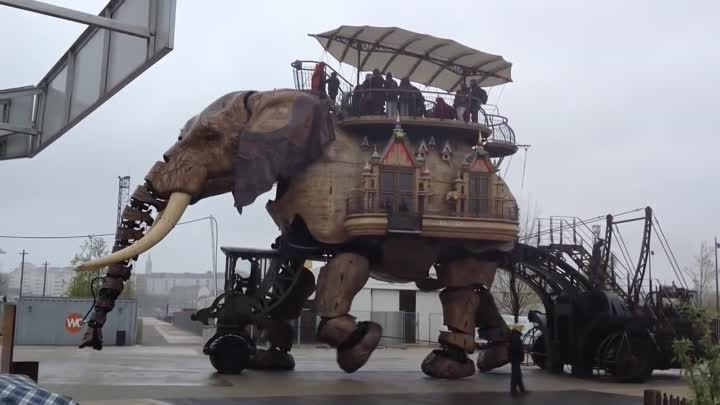
\includegraphics[width=0.8\textwidth]{from_master/mechEleph}
\caption{Механический слон}
\label{fig:mechEleph}
\end{figure}

К классу шагающих машин с дополнительными опорами относятся устройства, имеющие помимо дискретно взаимодействующих с опорной поверхностью шагающих движителей дополнительные механизмы, постоянно контактирующие с опорой \cite{Maloletov2015dinamica}. Необходимость в дополнительных опорах обычно возникает тогда, когда шагающих движителей недостаточно для обеспечения устойчивости машины. Чаще всего для этой цели шагающее транспортное средство оснащается колесной тележкой (рис. \ref{fig:Riksha},\ref{fig:steamMan})\cite{briskinSintezCiklovogoShagayushchego2011, Petr1986, Brisk2009,2014,2019,Pavl2013}.

\begin{figure}[H]
\centering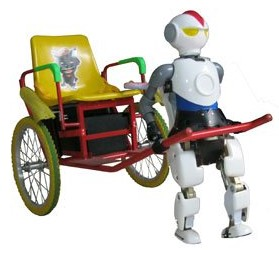
\includegraphics[width=0.6\textwidth]{from_master/Riksha}
\caption{Робот рикша}
\label{fig:Riksha}
\end{figure}

\begin{figure}[H]
\centering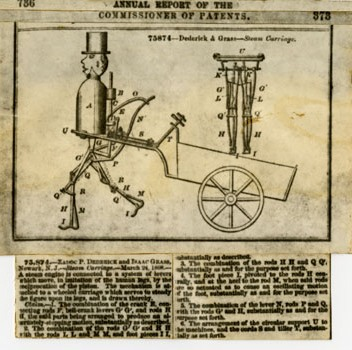
\includegraphics[width=0.9\textwidth]{from_master/steamMan}
\caption{Робот паровой человек}
\label{fig:steamMan}
\end{figure}

Такие машины обычно используются для демонстраций и отладки систем. Их применение бессмысленно, потому что они не обладают никакими преимуществами в сравнении с колесным роботом. 

Шагающие машины с циклическими движителями имеет несколько особенностей. Он характеризуется тем, что опорные точки шагающих механизмов движутся по одной и той же траектории относительно корпуса машины, и не решают проблемы адаптации к грунту и выбора точек постановки ног на землю. Такие машины имеют лучшую проходимость по сравнению с колесами меньшее сопротивление движению от земли, лучшее сцепление с основной поверхностью, большие возможности для снижения давления на грунт \cite{cruse2001control}. Примеры машин с циклическими движителями: (рис. \ref{fig:chebishev},\ref{fig:kuban}).

\begin{figure}[H]
\centering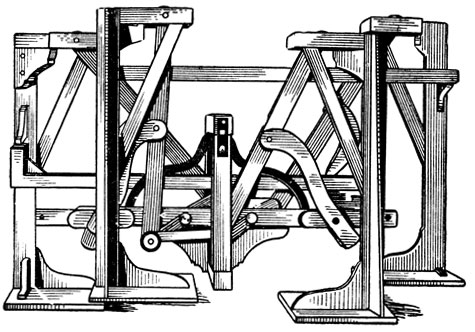
\includegraphics[width=0.8\textwidth]{from_master/chebishev}
\caption{Машина Чебышева}
\label{fig:chebishev}
\end{figure}

\begin{figure}[H]
\centering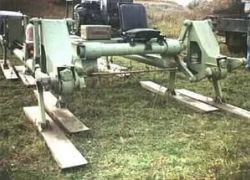
\includegraphics[width=0.9\textwidth]{from_master/kuban.jpg}
\caption{Робот ВолгГТУ Кубань}
\label{fig:kuban}
\end{figure}

Главной особенностью циклических шагающих машин является их простота конструкции и управление. 

Полноценная ходьба --- модификация предыдущего типа движителя и она дает наибольшие преимущества по сравнению с другими заявленными типами движителей. 

Данный способ передвижения позволяет использовать произвольный закон изменения скорости движения ноги как на этапе взаимодействия с землей, так и на этапе переноса. Такие машины обычно превосходят традиционные транспортные средства не только по грунтовой, но и по профильной проходимости. А их главным недостатком является сложность конструкции и системы управления. Это самый разнообразный и многообразный класс шаговых машин в мире, и многие из приведенных здесь примеров относятся к этому классу. 

Колесно-шагающими машинами традиционно называют класс устройств, в которых колеса шагающих движителей служат упорами. Такие машины могут работать в двух режимах: в режиме колесной машины и в режиме шагающей машины. В первом случае машина движется только с помощью колес. Во втором случае машина совершает шагающие движения, отрывая поочередно колеса от земли и переставляя их на новое место. В этом случае те, что соприкасаются с землей, могут либо блокироваться, либо поворачиваться в соответствии с движением опорных ног.
Известно несколько примеров (рис. \ref{fig:vniitm},\ref{fig:alduro},\ref{fig:athlete}) \cite{germann2001joystick}.

\begin{figure}[H].
\centering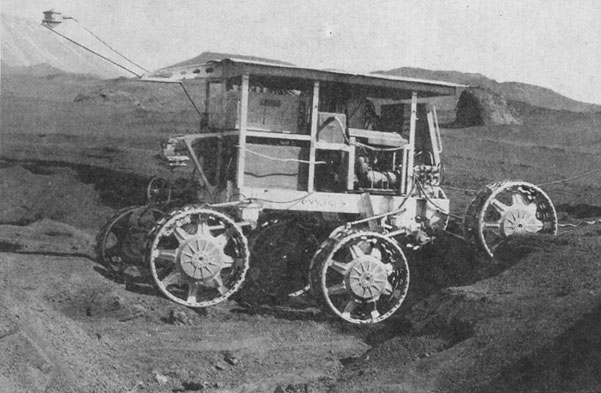
\includegraphics[width=0.9\textwidth]{from_master/vniitm}
\caption{VNIITM}
\label{fig:vniitm}
\end{figure}

\begin{figure}[H]
\centering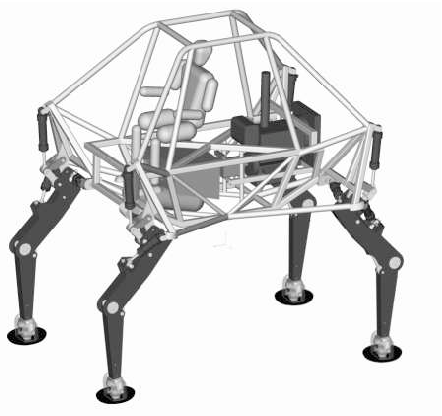
\includegraphics[width=0.9\textwidth]{from_master/alduro}
\caption{Робот Alduro}
\label{fig:alduro}
\end{figure}

\begin{figure}[H]
\centering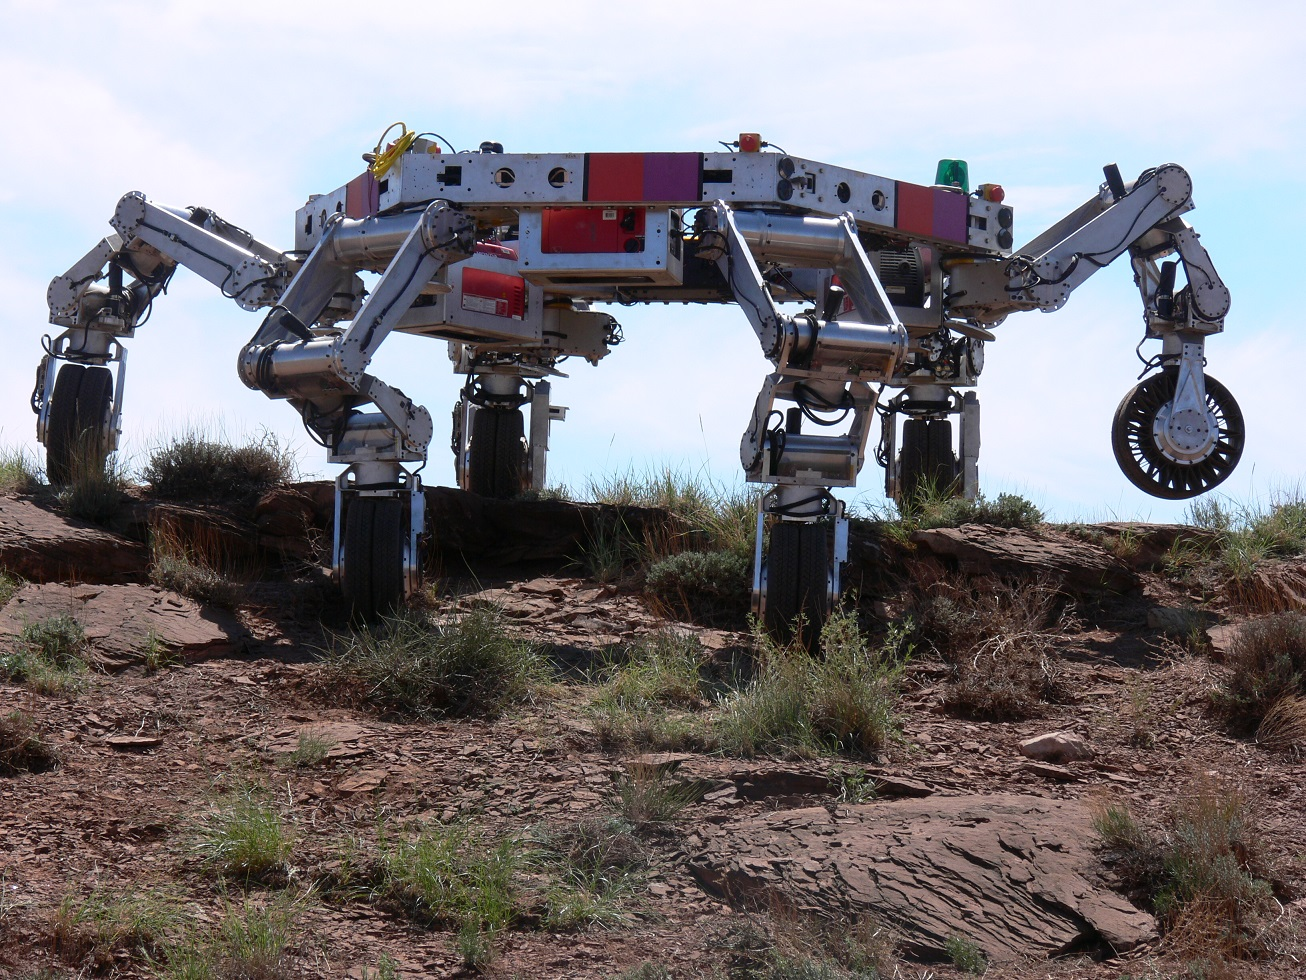
\includegraphics[width=0.8\textwidth]{from_master/athlete}
\caption{Робот Athlete}
\label{fig:athlete}
\end{figure}

Есть несколько машин, которые могут не только прыгать или бегать, но и шагать. Примеры следующие \cite{Pavl2013,volkovaModelirovanieDvizheniyaMnogozvennogo2013,bidgoly2010learning,yacunVibrorobotDlyaVertikalnogo2010} \pic{fig:bigDog}.

\begin{figure}[H]
    \centering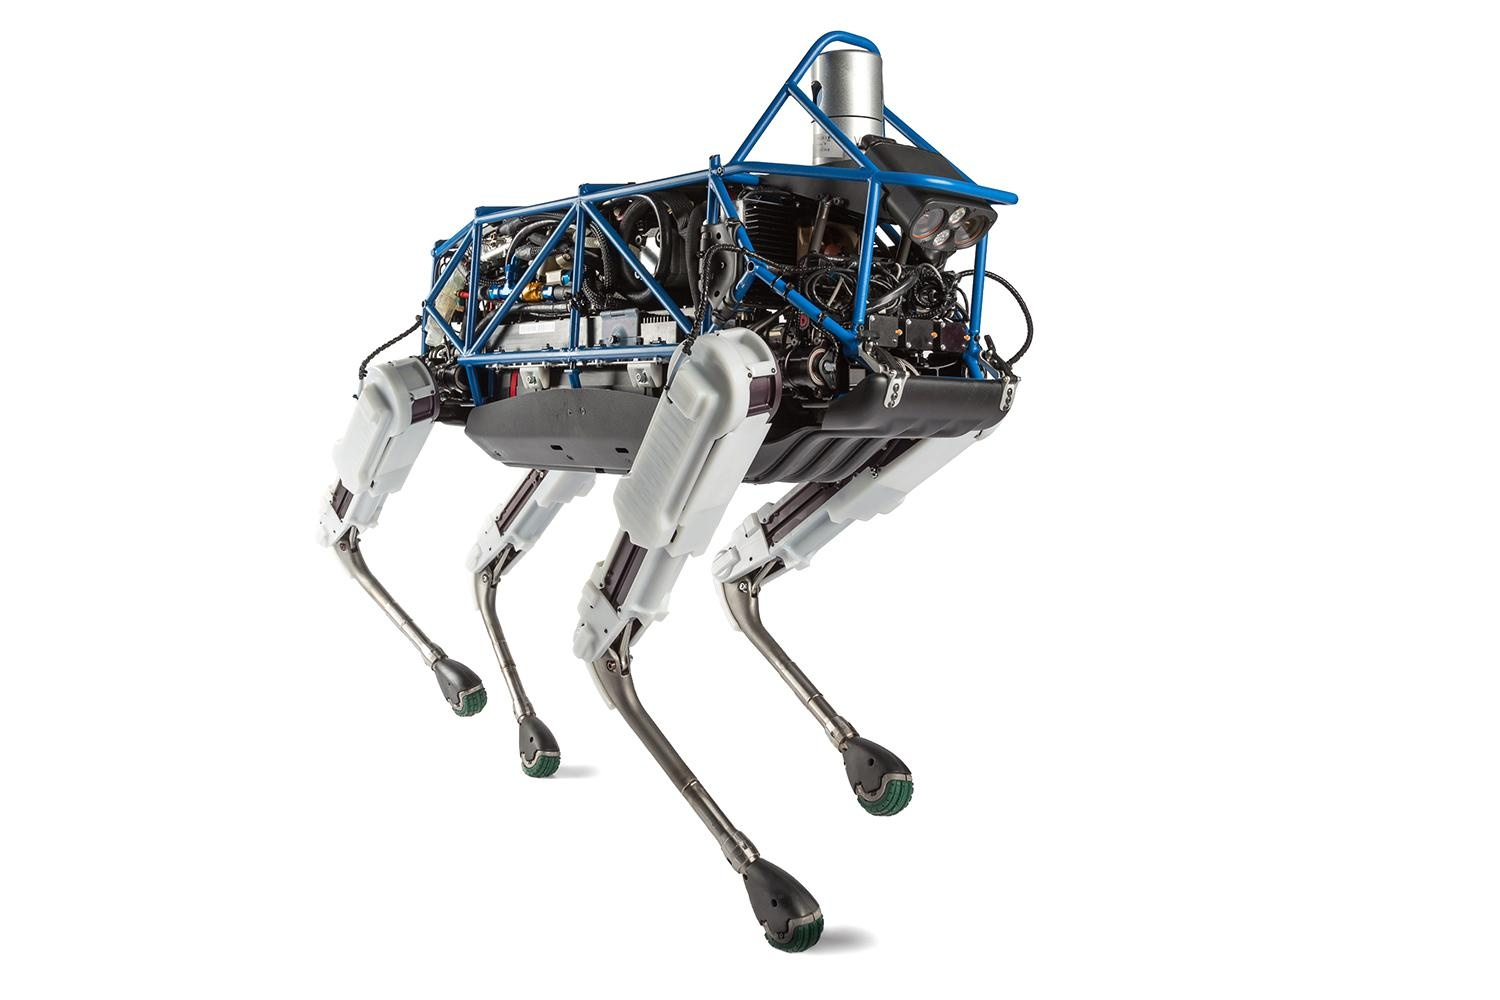
\includegraphics[width=0.9\textwidth]{from_master/bigDog}
\caption{BigDog}
\label{fig:bigDog}
\end{figure}

В соответствии с определением выше, к ползающим экскаваторам относится большинство таких машин, как шагающие экскаваторы \pic{fig:Esh6}. Несмотря на название "шагающие", такие машины перемещаются, поднимаясь по лестнице и ложась на опору при передвижении ног \cite{peters2010prototype,gradeckiySostoyaniePerspektivyRazvitiya2014,bidgoly2010learning}.

\begin{figure}[H]
\centering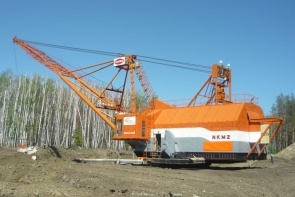
\includegraphics[width=0.8\textwidth]{from_master/Esh6}
\caption{Ползающий экскаватор Российского производства}
\label{fig:Esh6}
\end{figure}

 Специфика взаимодействия с опорной поверхностью и область применения лазающих машин настолько сильно отличаются, что сравнение их показателей (за исключением общетехнических) становится практически бессмысленным. Следует также отметить, что многие ползающие и лазающие роботы не имеют ног или какого-то их подобия, передвигаясь, например, за счет движений гибкого тела.

\begin{figure}[H]
\centering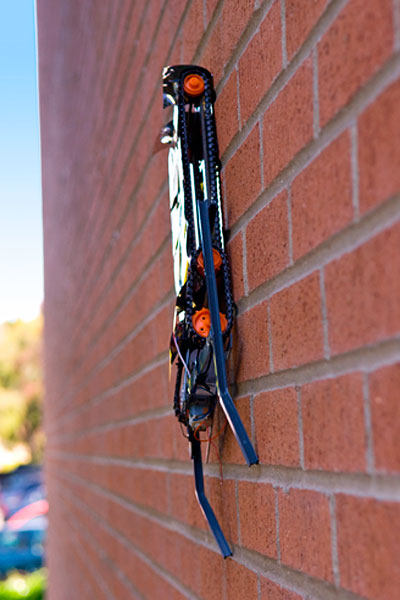
\includegraphics[width=0.45\textwidth]{from_master/brickwall}
\caption{BrickWall робот}
\label{fig:brickwall}
\end{figure}

\begin{figure}[H]
\centering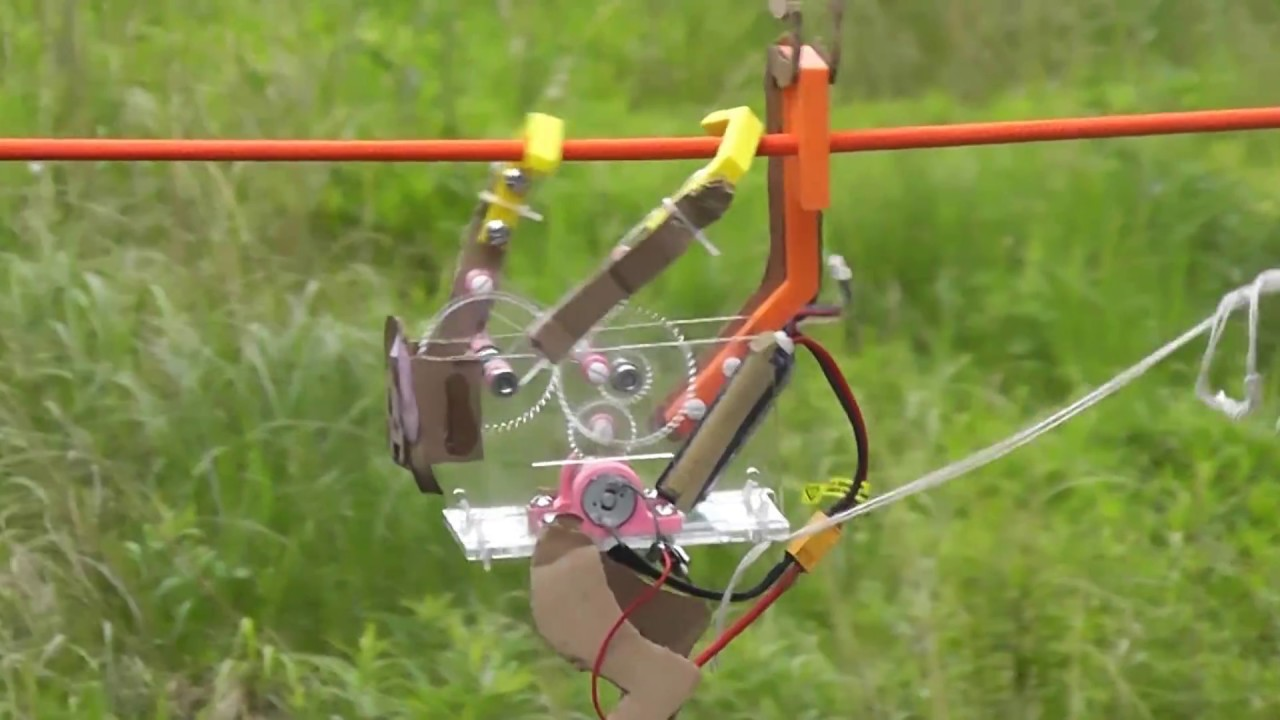
\includegraphics[width=0.8\textwidth]{from_master/ropeClimbing}
\caption{Робот, взбирающийся по канату}
\label{fig:ropeClimbing}
\end{figure}

Согласно этой классификации, робот, который используется в экспериментальной части, относится к категории <<Шагающие машины с циклическим действием движителей>>.

В течении разработки робототехнической системы, были спроектированы и изготовлены несколько прототипов шагающих роботов. Первым всемирно известным прототипом с подобной системой движения является робот RHex \cite{saranliRHexSimpleHighly2001} от Boston Dynamics. Группы ученных по всему миру развивали эту идею. Таким образом появились 3 новых подмножества. Роботы, которые умеют много сочленений. Системы, которые могут трансформироваться в колесных роботов и обратно. А также системы, которые являются псевдоколесными, то есть количество ног на одном моторе больше одной. Как итог, было решено добавить сочленение в разрабатываемую конструкцию. Также было оценен концепт с псевдоколесными роботами, так как это увеличивает проходимость по грунтам.

\section{Роботы, которые могут использоваться для исследования пещер}

Как было отмечено выше, одной из основных областей применения разрабатываемых роботов являются пещеры. Исследование пещер естественного происхождения является комплексной задачей, сопряженная со множественными трудностями \cite{Zhang2017a, Frumkin2019}. Деградация сенсоров \cite{Huang2019}, перебои в коммуникации между роботами из-за потери сигналов \cite{Vaquero2018, Thangavelautham2017}, сложный рельеф пещер \cite{Thangavelautham2017}, обилие грязи \cite{Baker2004}, жидких препятствий \cite{Morris2006}, требующие герметизацию корпуса, являются только малой частью встречаемых проблем в пещерах. 

В пещерах возможно встретить почти все типы поверхностей, с которыми приходится сталкиваться роботам в мире. Это и твердые поверхности: мрамор, кварц, базальт. Осадочные горные породы, такие как: мел, гипс, известняк. Часто встречаются водные препятствия — как лужи, так и целы залы, погруженные в воду. Особую опасность для человека вносят сифоны. Скользкие поверхности: лед, мох, глина, а так же разрушаемые поверхности — каменная гряда и паутина \cite{1960,1963,1969,1971}. Знание типов поверхностей и габаритов пещер влияет на типы сенсоров, которые будут установлены на робота и на на необходимую автономность робототехнической системы \cite{Mascarich2018a}. 

Для преодоления сложного рельефа различные роботы, робототехнические системы и типы движителей были предложены исследователями по всему миру \cite{Morris2006a}. Разрушение пещер нежелательно, поэтому роботы, которые для перемещения ломают породу, не рассмотрены в данном обзоре \cite{Semini2016}. Для исследования пещер используются, как наземных роботов, так и летающие аппараты, робототехнические комплексы. Из летающего транспорта это коптеры \cite{Papachristos2019,Scaramuzza2014,zinggMAVNavigationIndoor2010} и дирижабли \cite{Huang2019}. Дирижабль намного более автономен и может нести большую нагрузку. Наземных роботов очень много типов, но основными являются: шагающие \cite{Tan2016,Lynch2019} колесные \cite{Molyneaux2016,Vaquero2018}, трековые \cite{Reddy2015} и специфичные. Специфичные движители это движители роботов, которые не поддаются классификации, например змеевидные \cite{Ye2007,Borenstein2007}, шарообразные \cite{Thangavelautham2017,Dubowsky2008,Dang2019} и другие.

Для исследования пещер система роботов является самым эффективным способом разведки. Для использования систем роботов необходимо решать дополнительные задачи, как архитектурного характера, телекоммуникационного и управленческого. Обычно системы состоят из нескольких одинаковых роботов \cite{Vaquero2018}, связка – коптер и шагающий \cite{Chen2010,Cantelli2013}.

Ползающие роботы \cite{Schmidt2013} являются перспективными для исследования пещер по причине их высокой проходимости по узким и невысоким лазам. Например, известны ползающие роботы для исследования пещер, находящихся на других планетах \cite{Parness2017}. 

Важным критерием для выполнения задач разведки пещер, является способность перемещаться по вертикальным поверхностям, благодаря высокой адгезии с поверхностью. Это достигается следующими способами: существуют магнитный \cite{Lee2012,tavakoliOmniClimberOmnidirectionalLight2012,Kotay1996,Xu2017}, электрический \cite{Li2017}, негативного давления \cite{Lee2012,tavakoliOmniClimberOmnidirectionalLight2012,Papachristos2019}, пневматический или помощью присосок \cite{Nagakubo1994,Tlale2012}, зацепов ("когтей"), что иногда называют механической адгезией \cite{Parness2017,Bretl2006,SangbaeKim2005,Sintov2011}. Последний способ является самым применимым для пещер, так как стены рельефные. Рельефные стены с одной стороны препятствуют другим способам прикрепления к поверхности, а с другой стороны облегчают использование зацепов.

Навигация в пещерах является нетривиальной задачей, поэтому рассмотрены сенсоры и алгоритмы, а также архитектурные решения, которые используются в представленных выше роботах. Целесообразно рассмотреть работы в близких и смежных областях. К примеру, исследование трубопровода \cite{Savin2017} или завалов после техногенных катастроф. С точки зрения навигации основной проблемой является недостаток света, а также сильная неоднородность территории и обилие гранулированных поверхностей. Решение данной проблем сейчас уделено много внимания, одним из подтверждений данного тезиса является прошедшее соревнование DARPA Subterranean Challenge. В данном направлении используются как лазерные дальномеры (лидары), так и визуальные SLAM алгоритмы \cite{Mascarich2018a,Dang2019a,Fairfield2006,Chhaniyara2012}. С точки зрения архитектуры, наблюдается тенденция к модульности, а также к возможным защитам от потерь робота \cite{Miller2019,weiStudyMineRescue2009}. при работе роботов в группе один робот был потерян, то остальные роботы все равно должны передавать друг другу данные. 

Очень важно уметь правильно передвигать робота по сыпучим грунтам, следующие работы посвящены этим проблемам \cite{Tan2016,Savin2017,Chhaniyara2012,Tsounis2019, Li2009,Bjelonic2019,DeViragh2019,Buchanan2019}. Критичным критерием навигации является решение задачи в реальном времени.

Тип опорной поверхности является одним из ключевых параметров для адоптации управления робота. Зная тип опорной поверхности возможно оптимально построить маршрут по исследуемой территории. Следующие статьи и их обзоры покрывают основные способы решения данной задачи \cite{wuIntegratedGroundReaction2016,wuTactileSensingTerrainBased2020,luo_robotic_2017}.

Подведя итог, в данном разделе были представлены причины проблем, возникающие при разведке пещер роботами. Представлены причины, к примеру типы опорных поверхностей, которые влияют на подбор сенсоров и алгоритмов, а также сделаны выводы как это влияет на робототехническую систему. После этого показаны решения, предложенные исследователями по всему миру, связанные с навигацией, подбором движителя, выбором сенсоров и архитектурными решениями, дающие надежную систему. 

\section{Исследования роботов с цикловым движителем}
Одной из разновидностью роботов с цикловым движителем является гексаподы. Гексапод это разновидность мобильных шагающих роботов с 6 конечностями. Такая форма демонстрирует качественное поведение сороконожки. То есть, чаще всего роботы гексаподы --- биомиметические роботы, то есть роботы, вдохновленные природой.

Не смотря на это, существуют интересные попытки создать гибриды между колесными роботами и многоножками, чтобы получить <<лучшее из обоих миров>>.

Boston Dynamics RHex \cite{Altendorfer2001} - это шестиногий робот \pic{fig:rhex}. Данный робот является идейным вдохновителем множества разработок по всему миру, в том числе и для робота, разработанного автором диссертации. Независимо управляемые ноги создают специальные походки, которые перемещают его по неровной местности, такой как лестница, каменная гряда и т.д. Данный робот умеет прыгать. Форма ног обеспечивает плавность движений. Однако у робота есть и ряд недостатков. Прежде всего, это высокое энергопотребление, так как он содержит шесть двигателей. Кроме того, у этого робота есть некоторые трудности с управляемостью. 

\begin{figure}[H]
    \centering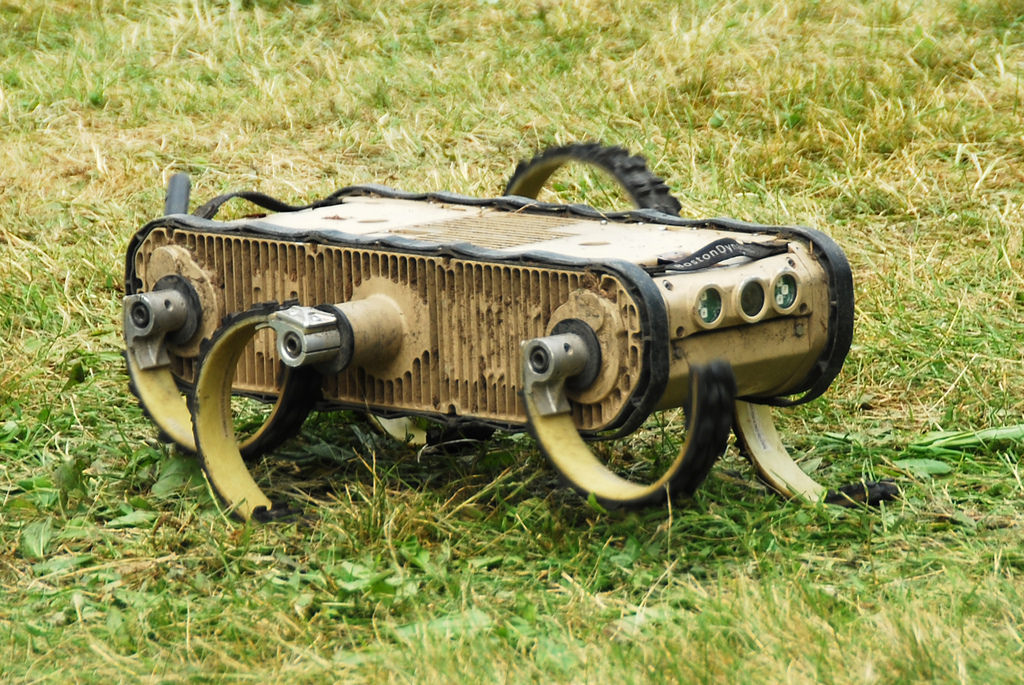
\includegraphics[width=0.9\textwidth]{from_master/rhex}\\
    \caption{Boston Dynamics робот RHex}
    \label{fig:rhex}
    \end{figure}

Gakken Mechamo Centipede \cite{millerExtremeMakeoverHeianera2008, Miller2019} - робот \pic{fig:gakken}, который имеет схожую кинематическую схему с СтриРусом. Стрирус это разработанный автором робот. Большое количество ног может обеспечить ему хорошую проходимость на пересеченной местности, и потеря ноги не будет критичной для робота. Однако это увеличило количество компонентов робота, что удорожает производство и техническое обслуживание. Минусом данной конструкции это малая длина педипулятора снижает возможности передвижения по пересеченной местности.
\begin{figure}[H]
    \centering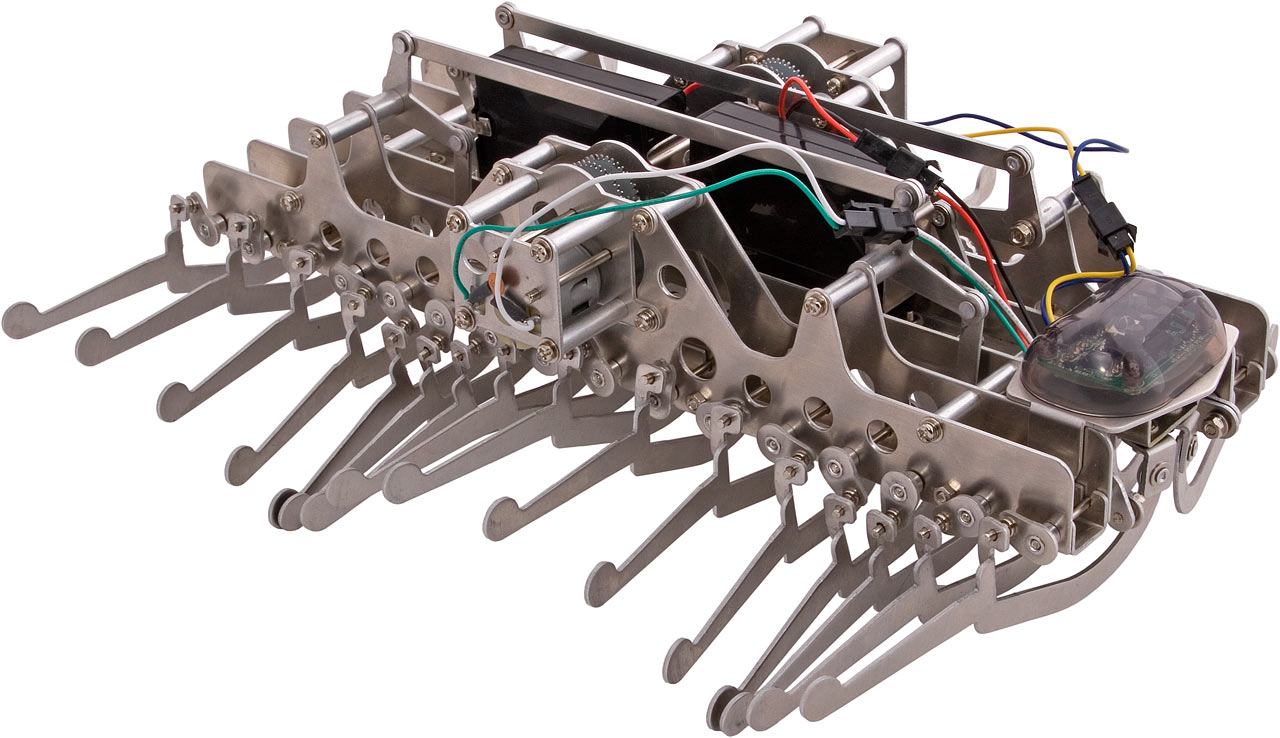
\includegraphics[width=0.8\textwidth]{from_master/gakken}\\
    \caption{Gakken Mechamo Centipede робот}
    \label{fig:gakken}
    \end{figure}

Quattroped и TurboQuad \cite{shenDesignLegwheelHybrid2009, Chen2014, Chen2017} --- это роботы, трансформирующие колеса в ноги \pic{quatro}. Когда он использует ноги, его кинематическая схема похожа на робота RHex, в случае режима работы колес он похож по управлению представляет собой четырёхколёсное транспортное средство. Данный инженерный прием обеспечивает высокую скорость на ровной местности, но конструкция робота становится конструкционно сложной, что снижает надежность системы. У робота 4 ноги, что делает его неустойчивым в некоторых ситуациях.

\begin{figure}[H]
    \begin{subfigure}{0.99\textwidth}
    \centering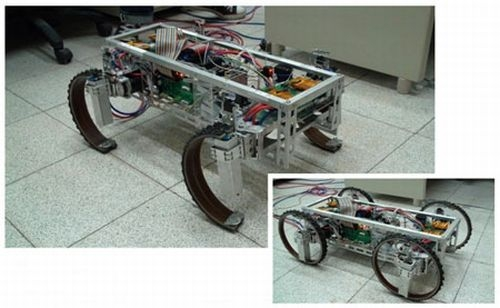
\includegraphics[width=0.9\textwidth]{from_master/quattroped}\\
    \caption{Quattroped robot}
    \label{fig:quattroped}
    \end{subfigure}

    \begin{subfigure}{0.99\textwidth}
    \centering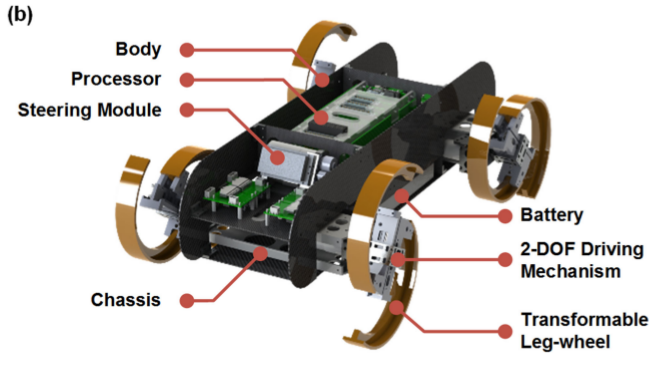
\includegraphics[width=0.9\textwidth]{from_master/turboquad}\\
    \caption{TurboQuad robot}
    \label{fig:turboquad}
    \end{subfigure}
    \caption{Quattroped семья роботов}
    \label{quatro}
    \end{figure}

Whegs \cite{schroerComparingCockroachWhegs2004} \pic{fig:whegs} использует стратегию локомоции, которая сочетает простоту колеса с преимуществами преодоления препятствий ногой. Робот обладает сегментированным телом, что позволяет ему при малой длине педипуляторов соперничать по проходимости с остальными представителями данного класса роботов. Сегментированность корпуса делает робота более сложным в изготовлении и управлении.

\begin{figure}[H]
\centering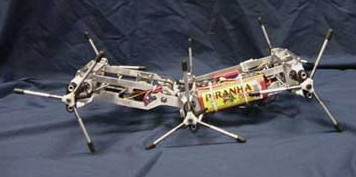
\includegraphics[width=0.9\textwidth]{from_master/whegs2.jpg}\\
\caption{Whegs II}
\label{fig:whegs}
\end{figure}

Сравнительный анализ между представленными выше роботами приведен в таблице \ref{tabular:robot_comparison}.
\begin{table}[H]
    \centering
\caption{Сравнительный анализ гексаподов}
\label{tabular:robot_comparison}
% \small
\begin{tabular}{l|c|c|c|c}
\toprule
\toprule
\rowcolor{Gray}
 Параметры, СИ & RHex & \makecell{Gakken \\ Mechamo\\ Centipede} &  \makecell{Quattroped} & \makecell{Whegs II}\\
 \hline
Длина, мм & 540 & 320 & 600 & 470 \\ 
  \rowcolor{LightGray}
 Ширина, мм & 200 & 140 & 190 & 360 \\
 Высота, мм & 127 & 100 & 140 & 50 \\
  \rowcolor{LightGray}
 Масса, кг & 8.2 & 1.1 & 8.6 & 3.86 \\ 
 Количество ног & 6 & 32 & 4 & 18 \\
  \rowcolor{LightGray}
 Высота ноги, мм & 175 & 50 & 175 & 100  \\
 Масса ноги, кг & 0.1 & 0.02 & 0.38 & 0.05 \\
  \rowcolor{LightGray}
 Скорость, м/с & 1.6 & 0.1 & 2 & 1.5 \\
\bottomrule
\bottomrule
\end{tabular}
% \end{center}
\end{table}

Все эти роботы, кроме Gakken Centipede, были созданы для разведки, в том числе и пространствах искусственного происхождения, поэтому значения параметров можно легко объяснить. Ширина должна быть меньше ширины дверного проема. Еще лучше, если ширина робота будет меньше 2/3 размера двери, и все прототипы удовлетворяют этому условию. При навигации внутри помещений длина также должна быть минимально возможной, иначе он не сможет передвигаться в коридорах и тесных помещениях. Масса зависит от других параметров. Высокая скорость не нужна в помещениях и опасных зонах. 

Роботы с цикловым движителем, такие как Boston Dynamics RHex \cite{Altendorfer2001}, Gakken Mechamo Centipede \cite{Miller2019}, Quattroped and TurboQuad \cite{Chen2011,Chen2014,Chen2017}, а так же Whegs \cite{schroerComparingCockroachWhegs2004} были рассмотрены. Рассмотрев других представителей выбранного класса роботов и определив причины таких параметров, было решено, что не следует превышать длину аппарата в один метр, в ширину --- меньше 70 см (стандартная ширина дверного проема). Иметь меньше 32 лапок и высота лапки должна быть больше 10 см. При большем количестве лапок начинаются большие проблемы с трением и кпд, что негативно сказывается на проходимости и энергопотреблении конструкции.


\section*{Вывод}
В ходе данного реферата мы исследовали классификацию мобильной шагающей робототехники, выявляя разнообразие и характеристики этого уникального класса роботов. Классификация позволила систематизировать различные типы шагающих роботов в соответствии с их основными характеристиками, от конструкции и приводов до типов ног и механизмов передвижения. Это помогло нам понять преимущества и ограничения каждого типа, а также определить их потенциальные применения в различных областях.

Мобильная шагающая робототехника имеет огромный потенциал и открывает новые возможности в области исследований, промышленности и помощи людям. Шагающие роботы могут эффективно передвигаться по сложным территориям, преодолевая препятствия, и быть полезными в задачах, где требуется подвижность и маневренность. Они могут применяться в исследованиях и разведке в труднодоступных или опасных местах, способствовать развитию автономных систем доставки и помогать людям с ограниченными возможностями.

Однако, несмотря на значительные прогрессивные достижения в этой области, мобильная шагающая робототехника все еще сталкивается с некоторыми вызовами и ограничениями. Это включает сложности в поддержании равновесия и стабильности, энергопотребление, ограниченную скорость и маневренность. Также существуют технические и программные сложности в разработке надежных алгоритмов управления и навигации для шагающих роботов.
